\documentclass[12pt,twoside]{article}

\textwidth 17cm \textheight 25cm \evensidemargin 0cm
\oddsidemargin 0cm \topmargin -2.5cm
\parindent 0pt
%\parskip \bigskipamount

\usepackage{graphicx}
\usepackage[dutch]{babel}
\usepackage{amssymb,amsthm,amsmath}
\usepackage[utf8]{inputenc}
\usepackage{nopageno}
\usepackage{pdfpages}
\usepackage{enumerate}
\usepackage{caption}
\usepackage{wrapfig}
\usepackage{pgf,tikz}
\usepackage{color}
\usetikzlibrary{arrows}
\usetikzlibrary{patterns}
\usepackage{fancyhdr}
\pagestyle{fancy}
\usepackage[version=3]{mhchem}
\usepackage{multicol}
\usepackage{fix-cm}
\usepackage{setspace}
\usepackage{mhchem}
\usepackage{xhfill}
\usepackage{parskip}
\usepackage{cancel}
\usepackage{mdframed}
\usepackage{url}

\newcommand{\todo}[1]{{\color{red} TODO: #1}}

\newcommand{\degree}{\ensuremath{^\circ}}
\newcommand\rad{\qopname\relax o{\mathrm{rad}}}

\newcommand\ggd{\qopname\relax o{\mathrm{ggd}}}

\def\LRA{\Leftrightarrow}%\mkern40mu}

\newcommand{\zrmbox}{\framebox{\phantom{EXE}}\phantom{X}}
\newcommand{\zrm}[1]{\framebox{#1}}

% environment oefening:
% houdt een teller bij die de oefeningen nummert, probeert ook de oefening op één pagina te houden
\newcounter{noefening}
\setcounter{noefening}{0}
\newenvironment{oefening}
{
  \stepcounter{noefening}
  \pagebreak[0]
  \begin{minipage}{\textwidth}
  \vspace*{0.7cm}{\large\bf Oefening \arabic{noefening}}
}{%
  \end{minipage}
}

\usepackage{calc}

% vraag
\reversemarginpar
\newcounter{punten}
\setcounter{punten}{0}
\newcounter{nvraag}
\setcounter{nvraag}{1}
\newlength{\puntwidth}
\newlength{\boxwidth}
\newcommand{\vraag}[1]{
\settowidth{\puntwidth}{\Large{#1}}
\setlength{\boxwidth}{1.5cm}
\addtolength{\boxwidth}{-\puntwidth}
{\large\bf Vraag \arabic{nvraag} \addtocounter{nvraag}{1}}\vspace*{-0.5cm}
{\marginpar{\color{lightgray}\fbox{\parbox{1.5cm}{\vspace*{1cm}\hspace*{\boxwidth}{\Large{#1}}}}}
\vspace*{0.5cm}}
\addtocounter{punten}{#1}}

% arulefill
\newcommand\arulefill[1][]{
  \ifstrempty{#1}{
    \leavevmode{
      \xrfill[-5pt]{0.3pt}[lightgray]
      \endgraf
    }
    \vspace*{0.2cm}
  }{
    \leavevmode{
      \xrfill[-5pt]{0.3pt}[lightgray]
      \endgraf
      \vspace*{0.2cm}
    }
    \foreach \n in {1,...,#1}{
      \leavevmode{
        \xrfill[-5pt]{0.3pt}[lightgray]
        \endgraf
        \vspace*{0.2cm}
      }
    }
  }
}
% \arules{n}
\newcommand{\arules}[1]{
\mbox{}
\color{lightgray}
%\vspace*{0.05cm}
\foreach \n in {1,...,#1}{
  \vspace*{0.75cm}
  \hrule height 0.3pt\hfill
}\color{black}\vspace*{0.2cm}}

% \arule{x}
\newcommand{\arule}[1]{
\color{lightgray}{\raisebox{-0.1cm}{\rule[-0.05cm]{#1}{0.3pt}}}\color{black}
}

% \abox{y}
\newcommand{\abox}[1]{
\fbox{
\begin{minipage}{\textwidth- 4\fboxsep}
\hspace*{\textwidth}\vspace{#1}
\end{minipage}
}
}

\newcommand{\ruitjes}[1]{
\definecolor{cqcqcq}{rgb}{0.85,0.85,0.85}
\hspace*{-2.5cm}
\begin{tikzpicture}[scale=1.04,line cap=round,line join=round,>=triangle 45,x=1.0cm,y=1.0cm]
\draw [color=cqcqcq, xstep=0.5cm, ystep=0.5cm] (0,-#1) grid (20.5,0);
\end{tikzpicture}
}


\newcommand{\assenstelsel}[5][1]{
\definecolor{cqcqcq}{rgb}{0.65,0.65,0.65}
\begin{tikzpicture}[scale=#1,line cap=round,line join=round,>=triangle 45,x=1.0cm,y=1.0cm]
\draw [color=cqcqcq,dash pattern=on 1pt off 1pt, xstep=1.0cm,ystep=1.0cm] (#2,#4) grid (#3,#5);
\draw[->,color=black] (#2,0) -- (#3,0);
\draw[shift={(1,0)},color=black] (0pt,2pt) -- (0pt,-2pt) node[below] {\footnotesize $1$};
\draw[color=black] (#3.25,0.07) node [anchor=south west] { x};
\draw[->,color=black] (0,#4) -- (0,#5);
\draw[shift={(0,1)},color=black] (2pt,0pt) -- (-2pt,0pt) node[left] {\footnotesize $1$};
\draw[color=black] (0.09,#5.25) node [anchor=west] { y};
\draw[color=black] (0pt,-10pt) node[right] {\footnotesize $0$};
\end{tikzpicture}
}

\newcommand{\getallenas}[3][1]{
\definecolor{cqcqcq}{rgb}{0.65,0.65,0.65}
\begin{tikzpicture}[scale=#1,line cap=round,line join=round,>=triangle 45,x=1.0cm,y=1.0cm]
\draw [color=cqcqcq,dash pattern=on 1pt off 1pt, xstep=1.0cm,ystep=1.0cm] (#2,-0.2) grid (#3,0.2);
\draw[->,color=black] (#2.25,0) -- (#3.5,0);
\draw[shift={(0,0)},color=black] (0pt,2pt) -- (0pt,-2pt) node[below] {\footnotesize $0$};
\draw[shift={(1,0)},color=black] (0pt,2pt) -- (0pt,-2pt) node[below] {\footnotesize $1$};
\draw[color=black] (#3.25,0.07) node [anchor=south west] {$\mathbb{R}$};
\end{tikzpicture}
}

\newcommand{\visgraad}[1]{\begin{tabular}{p{0.5cm}|p{#1}}&\\\hline\\\end{tabular}}

\newcommand{\tekenschema}[2]{\begin{tabular}{p{0.5cm}|p{#1}}&\\\hline\\[#2]\end{tabular}}

% schema van Horner
\newcommand{\schemahorner}{
\begin{tabular}{p{0.5cm}|p{7cm}}
&\\[1.5cm]
\hline\\
\end{tabular}}

% geef tabular iets meer ruimte
\setlength{\tabcolsep}{14pt}
\renewcommand{\arraystretch}{1.5}

\newcommand{\toets}[3]{
\thispagestyle{plain}
\vspace*{-2.5cm}
\begin{tikzpicture}[remember picture, overlay]
    \node [shift={(15.25 cm,-1.6cm)}] {%
        \includegraphics[width=1.8cm]{/home/ppareit/kaa1415/logokaavelgem.png}%
    };%
\end{tikzpicture}

\begin{tabular}{|llc|c|}
\hline
\vspace*{-0.5cm}
&&&\\
Naam & \arule{4cm} & {\Large\bf KA AVELGEM} & \\
\vspace*{-0.75cm}
&&&\\
Klas & \arule{4cm} & {\Large\bf 20...-...-...} & \\
\hline
\vspace*{-0.75cm}
&&&\\
Toets & {\bf #2} & {\large\bf #1} & Beoordeling\\
\vspace*{-0.75cm}
&&&\\
Onderwerp & \multicolumn{2}{l|}{\bf #3} &\\
\hline
\end{tabular}
}

\newcommand{\oefeningen}[1]{

\fancyhead[LE, RO]{\vspace{0.5cm} #1}
%\thispagestyle{plain}

{\bf \Large \centering Oefeningen: #1}

}

\raggedbottom

\newcommand\dom{\qopname\relax o{\mathrm{dom}}}
\newcommand\ber{\qopname\relax o{\mathrm{ber}}}

\newcommand\mC{\qopname\relax o{\mathrm{mC}}}
\newcommand\uC{\qopname\relax o{\mathrm{{\mu}C}}}
\newcommand\C{\qopname\relax o{\mathrm{C}}}

\newcommand\W{\qopname\relax o{\mathrm{W}}}
\newcommand\kW{\qopname\relax o{\mathrm{kW}}}
\newcommand\kWh{\qopname\relax o{\mathrm{kWh}}}


\newcommand\V{\qopname\relax o{\mathrm{V}}}
\newcommand\ohm{\qopname\relax o{\mathrm{\Omega}}}
\newcommand\kohm{\qopname\relax o{\mathrm{k\Omega}}}


\newcommand\N{\qopname\relax o{\mathrm{N}}}

\newcommand\Nperkg{\qopname\relax o{\mathrm{N/kg}}}

\newcommand\Nperm{\qopname\relax o{\mathrm{N/m}}}

\newcommand\gpermol{\qopname\relax o{\mathrm{g/mol}}}


\newcommand\kgperm{\qopname\relax o{\mathrm{kg/m}}}
\newcommand\kgperdm{\qopname\relax o{\mathrm{kg/dm}}}
\newcommand\gpercm{\qopname\relax o{\mathrm{g/cm}}}
\newcommand\gperml{\qopname\relax o{\mathrm{g/ml}}}


\newcommand{\mA}{\;\mbox{mA}}
\newcommand{\A}{\;\mbox{A}}
\newcommand{\MA}{\;\mbox{MA}}

\newcommand{\us}{\;\mu\mbox{s}}
\newcommand\s{\qopname\relax o{\mathrm{s}}}

\newcommand\h{\qopname\relax o{\mathrm{h}}}

\newcommand{\mpers}{\;\mbox{m/s}}
\newcommand{\kmperh}{\;\mbox{km/h}}
\newcommand{\kmpermin}{\;\mbox{km/min}}
\newcommand{\kmpers}{\;\mbox{km/s}}

\newcommand{\mph}{\;\mbox{mph}}

\newcommand{\Hz}{\;\mbox{Hz}}

\newcommand\Gm{\qopname\relax o{\mathrm{Gm}}}
\newcommand\Mm{\qopname\relax o{\mathrm{Mm}}}
\newcommand\km{\qopname\relax o{\mathrm{km}}}
\newcommand\hm{\qopname\relax o{\mathrm{hm}}}
\newcommand\dam{\qopname\relax o{\mathrm{dam}}}
\newcommand\m{\qopname\relax o{\mathrm{m}}}
\newcommand\dm{\qopname\relax o{\mathrm{dm}}}
\newcommand\cm{\qopname\relax o{\mathrm{cm}}}
\newcommand\mm{\qopname\relax o{\mathrm{mm}}}
\newcommand\um{\qopname\relax o{\mathrm{{\mu}m}}}
\newcommand\nm{\qopname\relax o{\mathrm{nm}}}


\newcommand\Gg{\qopname\relax o{\mathrm{Gg}}}
\newcommand\Mg{\qopname\relax o{\mathrm{Mg}}}
\newcommand\kg{\qopname\relax o{\mathrm{kg}}}
\newcommand\hg{\qopname\relax o{\mathrm{hg}}}
\renewcommand\dag{\qopname\relax o{\mathrm{dag}}}
\newcommand\g{\qopname\relax o{\mathrm{g}}}
\newcommand\dg{\qopname\relax o{\mathrm{dg}}}
\newcommand\cg{\qopname\relax o{\mathrm{cg}}}
\newcommand\mg{\qopname\relax o{\mathrm{mg}}}
\newcommand\ug{\qopname\relax o{\mathrm{{\mu}g}}}
\renewcommand\ng{\qopname\relax o{\mathrm{ng}}}

\newcommand\ton{\qopname\relax o{\mathrm{ton}}}

\newcommand\Gl{\qopname\relax o{\mathrm{Gl}}}
\newcommand\Ml{\qopname\relax o{\mathrm{Ml}}}
\newcommand\kl{\qopname\relax o{\mathrm{kl}}}
\newcommand\hl{\qopname\relax o{\mathrm{hl}}}
\newcommand\dal{\qopname\relax o{\mathrm{dal}}}
\renewcommand\l{\qopname\relax o{\mathrm{l}}}
\newcommand\dl{\qopname\relax o{\mathrm{dl}}}
\newcommand\cl{\qopname\relax o{\mathrm{cl}}}
\newcommand\ml{\qopname\relax o{\mathrm{ml}}}
\newcommand\ul{\qopname\relax o{\mathrm{{\mu}l}}}
\newcommand\nl{\qopname\relax o{\mathrm{nl}}}

\newcommand\MJ{\qopname\relax o{\mathrm{MJ}}}
\newcommand\kJ{\qopname\relax o{\mathrm{kJ}}}
\newcommand\J{\qopname\relax o{\mathrm{J}}}

\newcommand\T{\qopname\relax o{\mathrm{T}}}
\newcommand\uT{\qopname\relax o{\mathrm{{\mu}T}}}

\newcommand\grC{\qopname\relax o{\mathrm{{\degree}C}}}

\newcommand\K{\qopname\relax o{\mathrm{K}}}
\newcommand\calperK{\qopname\relax o{\mathrm{cal/K}}}

\newcommand\hPa{\qopname\relax o{\mathrm{hPa}}}
\newcommand\Pa{\qopname\relax o{\mathrm{Pa}}}

\newcommand\dB{\qopname\relax o{\mathrm{dB}}}

\newcommand{\EE}[1]{\cdot 10^{#1}}

\onehalfspacing

%\singlespacing
%\onehalfspacing
%\doublespacing

%\setlength{\headsep}{0cm}

\newenvironment{exlist}[1] %
{ \begin{multicols}{#1}
  \begin{enumerate}[(a)]
    \setlength{\itemsep}{0.8em} }
{ \end{enumerate}
  \end{multicols} }




\usepackage{pgfplots}

%\renewcommand{\rmdefault}{phv} % Arial
%\renewcommand{\sfdefault}{phv} % Arial

\begin{document}

\thispagestyle{empty}
\begin{center}
  \begin{mdframed}
  \centering
  \fontsize{50}{70}\selectfont De normale verdeling
  \end{mdframed}
  \vfill
  
\includegraphics[width=0.8\textwidth]{normal}
  \vfill
\end{center}
%\vfill
\vspace*{-2cm}
\subsection*{Doelstellingen}
{\singlespacing
Je \hfill  {\scriptsize(LP 2005/069, LI 2.3.2, ET16)}
\begin{itemize}
  \item kan aan de hand van voorbeelden, in betekenisvolle situaties, gebruik maken van de normale verdeling (met de bijhorende klokcurve) als model van een reeks statistische gegevens.
  \item kan het gemiddelde en de standaardafwijking gebruiken als karakteristieken van een normale verdeling en deze kengetallen ook grafisch interpreteren.
\end{itemize}

\thispagestyle{empty}
\mbox{}
\newpage
\clearpage
\thispagestyle{empty}
\mbox{}
\newpage
\clearpage
\pagenumbering{arabic} 

\fancyhead[RO,LE]{De normale verdeling}
\fancyhead[RE,LO]{}

\onehalfspacing

\section{Inleiding}

Vorig jaar heeft een bekend kledingmerk een statistische onderzoek verricht naar de lichaamsafmetingen van vrouwen. Dit om beter passende kledij te ontwikkelen. Voor het onderzoek werden bij 160 willekeurig gekozen vrouwen 11 lichamelijke kenmerken gemeten. De resultaten voor de lichaamslengte vind je in onderstaande dataset:

\begin{center}  
\singlespacing
\scriptsize
166.38
165.46
163.8
169.75
168.27
167.44
165.56
165.75
166.13
165.41
168.69
166.14
166.68
165.99
164.67
164.26
165.05
168.58
166.6
168.13
161.26
167.9
165.5
164.28
163.38
167.01
164.52
162.84
166.19
165.3
167.28
165.32
167.57
168.4
163.71
166.59
167.85
164.36
166.83
166.05
163.94
164.85
168
166.2
167.14
162.93
169.47
166.84
169.08
166.58
166.53
165.85
167.04
168.66
169.41
170.1
164.27
163.26
164.8
164.49
164.54
169.09
165.39
164.29
164.86
166.14
166.49
167.32
164.38
166.54
170.92
163.83
167.41
168.67
168.88
167.66
165.89
166.17
165.4
166.27
166.32
162.55
169.33
168.61
167.09
164.28
165.94
164.22
165.43
164.07
167.75
163.86
167.35
163.78
167.08
167.82
164.48
166.06
164.62
167.08
169.12
166.27
163.5
168.67
164.44
165.63
164.62
165.56
166.86
164.41
166.95
167.41
167.43
166.06
166.73
168.92
167.56
168.81
166.89
164.34
164.3
165.24
168.7
165.63
164.34
165.41
165.71
165.58
166.49
165.61
167.36
169.06
164.41
167.77
167.16
168.1
164.56
162.29
166.1
164.13
159.48
167.98
162.43
167.57
167.25
163.9
168.06
160.94
164.24
163.75
168.11
162.9
164.1
165.36
165.81
166.31
163.96
166.32
165.45
165.06
\end{center}

Deze gegevens zeggen uiteraard niet veel. Omdat de gegevens \arule{4cm} zijn, verdelen we ze in 10 klassen en plaatsen we ze in volgende \arule{4cm}:

\begin{center}
\definecolor{cqcqcq}{rgb}{0.75,0.75,0.75}
\begin{tikzpicture}[yscale=0.2, line cap=round,line join=round,>=triangle 45,x=1.0cm,y=1.0cm]
\draw [color=cqcqcq,dash pattern=on 7pt off 7pt, xstep=2.0cm,ystep=10.0cm] (159.01,-4.38) grid (171.44,44.53);
\draw[->,color=black] (159.01,0) -- (171.44,0);
\foreach \x in {160,162,164,166,168,170}
\draw[shift={(\x,0)},color=black] (0pt,2pt) -- (0pt,-2pt) node[below] {\footnotesize $\x$};
\clip(159.01,-4.38) rectangle (171.44,44.53);
\draw[line width=1.2pt,fill=black,fill opacity=0.3] (159.48,0) rectangle (160.63,1);
\draw[line width=1.2pt,fill=black,fill opacity=0.3] (160.63,0) rectangle (161.77,2);
\draw[line width=1.2pt,fill=black,fill opacity=0.3] (161.77,0) rectangle (162.91,5);
\draw[line width=1.2pt,fill=black,fill opacity=0.3] (162.91,0) rectangle (164.06,13);
\draw[line width=1.2pt,fill=black,fill opacity=0.3] (164.06,0) rectangle (165.2,31);
\draw[line width=1.2pt,fill=black,fill opacity=0.3] (165.2,0) rectangle (166.35,40);
\draw[line width=1.2pt,fill=black,fill opacity=0.3] (166.35,0) rectangle (167.49,31);
\draw[line width=1.2pt,fill=black,fill opacity=0.3] (167.49,0) rectangle (168.63,19);
\draw[line width=1.2pt,fill=black,fill opacity=0.3] (168.63,0) rectangle (169.78,16);
\draw[line width=1.2pt,fill=black,fill opacity=0.3] (169.78,0) rectangle (170.92,2);
\end{tikzpicture}
\end{center}

\begin{minipage}{\textwidth}
We laten {\em GeoGebra} ook de volgende \arule{4cm} uitrekenen, we vinden volgende resultaten:

%\begin{center}
  \begin{tabular}{c l|r}
      \arule{4cm} & $n$ & 160\\
      \arule{4cm} & $\bar{x}$ & 166.03\\
      \arule{4cm} & $s$ & 1.94\\
                    & min & 159.5\\
                    & $Q_1$ & 164.5\\
                    & Med & 166.07\\
                    & $Q_3$ & 167.4\\
                    & max & 170.9\\
  \end{tabular}
%\end{center}
\end{minipage}

Het histogram geeft ons de mogelijkheid een tweede grafiek te tekenen, de {\bf frequentiepolygoon}. Deze verkrijgen we door de middens van de bovenste zijden van alle rechthoeken met elkaar te verbinden.

\begin{oefening}
Teken op het bovenstaand histogram het frequentiepolygoon.
\end{oefening}

De ontstane kromme is een {\bf klokvormige kromme}, met een symmetrieas door het gemiddelde. Hoe hoger het aantal klassen, hoe vloeiender de kromme wordt. In de volgende figuur werd dit gedaan in de limiet (er werd aangenomen dat het onderzoek bij oneindig veel vrouwen werd uitgevoerd):

\begin{center}
\definecolor{cqcqcq}{rgb}{0.75,0.75,0.75}
\begin{tikzpicture}[yscale=0.2, line cap=round,line join=round,>=triangle 45,x=1.0cm,y=1.0cm]
\draw [color=cqcqcq,dash pattern=on 7pt off 7pt, xstep=2.0cm,ystep=10.0cm] (159.01,-4.38) grid (171.44,30.53);
\draw[->,color=black] (159.01,0) -- (171.44,0);
\foreach \x in {160,162,164,166,168,170}
\draw[shift={(\x,0)},color=black] (0pt,2pt) -- (0pt,-2pt) node[below] {\footnotesize $\x$};
\clip(159.01,-4.38) rectangle (171.44,32);
\draw[line width=1.6pt, smooth,samples=100,domain=150:176] plot(\x,{160*exp((-(((\x)-166)/2.05)^2)/2)/(sqrt(2*3.14)*abs(2.05))});
\end{tikzpicture}
\end{center}

\begin{oefening}
Waar ligt de symmetrieas in ons voorbeeld? \arule{4cm} Teken deze op bovenstaande grafiek.
\end{oefening}

Dit is een typisch voorbeeld van een {\bf normale verdeling}. Dergelijke kromme kan beschreven worden door een functie $f(x)$ die in de context van de statistiek een {\bf dichtheidsfunctie} genoemd word. In ons voorbeeld wordt het functievoorschrift

$$f(x)=\dfrac{1}{1.94\sqrt{2\pi}}\;e^{-\dfrac{1}{2}\left(\dfrac{x-166.03}{1.94}\right)^2}\;.$$

\pagebreak
\section{Algemeen}

\begin{minipage}{0.5\textwidth}
De grafieken van gegevens die een normale verdeling hebben, zijn steeds
\begin{itemize}
  \item symmetrische
  \item ééntoppige
  \item klokvormige
\end{itemize}
krommen. Ze hebben allemaal dezelfde globale vorm, zie rechts.
\end{minipage}
\begin{minipage}{0.5\textwidth}
\begin{center}
\definecolor{cqcqcq}{rgb}{0.75,0.75,0.75}
\begin{tikzpicture}[yscale=8, line cap=round,line join=round,>=triangle 45,x=1.0cm,y=1.0cm]
\draw [color=cqcqcq,dash pattern=on 1pt off 1pt, xstep=0.5cm,ystep=0.2cm] (-3.4,-0.1) grid (3.4,0.65);
\draw[->,color=black] (-3.5,0) -- (3.5,0);
\foreach \x in {-3,-2,-1,1,2,3}
\draw[shift={(\x,0)},color=black] (0pt,2pt) -- (0pt,-2pt) node[below] {\footnotesize $\x$};
\draw[->,color=black] (0,-0.1) -- (0,0.65);
\foreach \y in {0.2,0.4,0.6}
\draw[shift={(0,\y)},color=black] (2pt,0pt) -- (-2pt,0pt) node[left] {\footnotesize $\y$};
\clip(-3.5,-0.1) rectangle (3.5,0.65);
\draw[line width=1.6pt, smooth,samples=100,domain=-3.5:3.5] plot(\x,{exp((-((\x))^2)/2)/(sqrt(2*3.1415926535))});
\end{tikzpicture}
\end{center}
\end{minipage}

Vergelijk nu het voorschrift van $f(x)$ uit ons initieel voorbeeld, dat waarbij de lengtes van 160 dames werd gemeten, met de centrumgetallen en de spreidingsmaten van dat voorbeeld om een algemeen voorschrift af te leiden voor een normale verdeling:

\begin{oefening}
Vul de normale verdeling aan met $\bar{x}$ en $s$

$$f(x)=\dfrac{1}{\arule{1cm}{\sqrt{2\pi}}}\;e^{-\dfrac{1}{2}\left(\dfrac{x-\arule{1cm}}{\arule{1cm}}\right)^2}\;.$$
\end{oefening}

Wanneer een enquête wordt uitgevoerd, wordt steeds gewerkt met een steekproef. Voor deze steekproef berekenen we dan het gemiddelde $\bar{x}$ en de standaardafwijking $s$.

\begin{oefening}
Een steekproef wordt steeds genomen als een klein deel uit de \arule{5cm}. Waarom doen we dit?
\arules{3}
\end{oefening}

Indien de omvang van de steekproef voldoende groot is, veralgemenen we deze resultaten voor de volledige populatie. De populatie heeft echter zelf ook een gemiddelde en een standaardafwijking. Die kunnen lichtjes verschillen van deze van de steekproef. Om de twee niet te verwarren wordt een andere notatie toegekend:

\begin{center}
\begin{tabular}{c|c|c}
& Steekproef & Populatie\\
\hline
Gemiddelde & $\bar{x}$ & $\mu$ (mu)\\
Standaardafwijking & $s$ & $\sigma$ (sigma)\\
\end{tabular}
\end{center}

Zo wordt het algemene voorschrift voor een normaal verdeelde populatie:

$$f(x)=\dfrac{1}{\sigma{\sqrt{2\pi}}}\;e^{-\dfrac{1}{2}\left(\dfrac{x-\mu}{\sigma}\right)^2}$$

Omdat dit voorschrift volledig bepaald is door het gemiddelde $\mu$ en de standaardafwijking $\sigma$, noteren we dit kort als $N(\mu,\sigma)$.

\pagebreak
\section{Voorbeelden van normaal verdeelde gegevens}

De normale verdeling is zonder twijfel de meest gebruikte verdeling in de statistiek. Van heel wat gegevens is immers geweten dat ze normaal verdeeld zijn:
\begin{itemize}
  \item lengte en gewicht van mensen en dieren
  \item het IQ
  \item de effectieve inhoud van machinaal gevulde verpakkingen
  \item sportprestaties
\end{itemize}
\begin{oefening} Geef zelf een voorbeeld van normaal verdeelde gegevens:
\begin{itemize}
  \item \dotfill
\end{itemize}
\end{oefening}

Men mag hier echter niet uit besluiten dat alles normaal verdeeld zou zijn. Typische voorbeelden van niet-normaal verdeelde gegevens zijn:
\begin{itemize}
  \item de leeftijd bij het overlijden van mens of dier
  \item het inkomen
\end{itemize}
\begin{oefening} Geef zelf een voorbeeld van niet normaal verdeelde gegevens:
\begin{itemize}
  \item \dotfill
\end{itemize}
\end{oefening}

\begin{center}
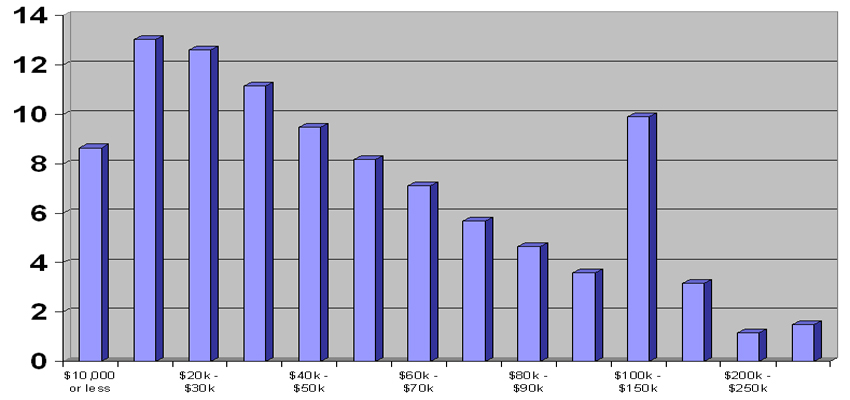
\includegraphics[width=\textwidth]{Income-curve}
\end{center}

\newpage
\section{Grafische betekenis van $\mu$ en $\sigma$}

\subsection{Grafische betekenis van $\mu$}

We laten in het functievoorschrift van de normale verdeling
$$f(x)=\dfrac{1}{\sigma{\sqrt{2\pi}}}\;e^{-\dfrac{1}{2}\left(\dfrac{x-\mu}{\sigma}\right)^2}$$
het gemiddelde $\mu$ variëren, terwijl de standaardafwijking $\sigma$ constant houden ($\sigma=1$). Hieronder zie je de grafieken voor verschillende waarden van $\mu$:
\begin{center}
\definecolor{cqcqcq}{rgb}{0.75,0.75,0.75}
\begin{tikzpicture}[yscale=8,line cap=round,line join=round,>=triangle 45,x=1.0cm,y=1.0cm]
\draw [color=cqcqcq,dash pattern=on 1pt off 1pt, xstep=1.0cm,ystep=0.1cm] (-6,-0.1) grid (6,0.6);
\draw[->,color=black] (-6,0) -- (6,0);
\foreach \x in {-6,-5,-4,-3,-2,-1,1,2,3,4,5}
\draw[shift={(\x,0)},color=black] (0pt,2pt) -- (0pt,-2pt) node[below] {\footnotesize $\x$};
\draw[->,color=black] (0,-0.1) -- (0,0.6);
\foreach \y in {,0.2,0.3,0.4,0.5}
\draw[shift={(0,\y)},color=black] (2pt,0pt) -- (-2pt,0pt) node[left] {\footnotesize $\y$};
\clip(-6,-0.1) rectangle (6,0.6);
\draw[line width=1.6pt, smooth,samples=100,domain=-6.0:6.0] plot(\x,{exp((-((\x))^2)/2)/(sqrt(2*3.1415926535)*abs(1))});
\draw[line width=1.6pt, smooth,samples=100,domain=-6.0:6.0] plot(\x,{exp((-((\x)+3)^2)/2)/(sqrt(2*3.1415926535)*abs(1))});
\draw[line width=1.6pt, smooth,samples=100,domain=-6.0:6.0] plot(\x,{exp((-((\x)-2)^2)/2)/(sqrt(2*3.1415926535)*abs(1))});
\draw (-5.5,0.38) node[anchor=north west] {$\mu=-3$};
\draw (0.3,0.5) node[anchor=north west] {$\mu=0$};
\draw (2.82,0.35) node[anchor=north west] {$\mu=2$};
\end{tikzpicture}
\end{center}

We merken dat de grafieken van al deze normale verdelingen met constante $\sigma=1$ op een verschuiving evenwijdig met de $x$-as met $\mu$ eenheden na gelijk zijn.

\begin{oefening}
Voor welke $x$-waarde vinden we steeds de top van de klokvormige kromme?
\arules{1}
\end{oefening}

\subsection{Grafische betekenis van $\sigma$}

We laten nu in het functievoorschrift 
$$f(x)=\dfrac{1}{\sigma{\sqrt{2\pi}}}\;e^{-\dfrac{1}{2}\left(\dfrac{x-\mu}{\sigma}\right)^2}$$
de standaardafwijking $\sigma$ variëren, terwijl we het gemiddelde $\mu$ constant houden op $\mu=0$.

\begin{center}
\definecolor{cqcqcq}{rgb}{0.75,0.75,0.75}
\begin{tikzpicture}[yscale=8, line cap=round,line join=round,>=triangle 45,x=1.0cm,y=1.0cm]
\draw [color=cqcqcq,dash pattern=on 1pt off 1pt, xstep=2.0cm,ystep=0.2cm] (-5.5,-0.1) grid (5.5,0.85);
\draw[->,color=black] (-6,0) -- (7,0);
\foreach \x in {-6,-4,-2,2,4,6}
\draw[shift={(\x,0)},color=black] (0pt,2pt) -- (0pt,-2pt) node[below] {\footnotesize $\x$};
\draw[->,color=black] (0,-0.1) -- (0,0.9);
\foreach \y in {,0.2,0.4,0.6,0.8}
\draw[shift={(0,\y)},color=black] (2pt,0pt) -- (-2pt,0pt) node[left] {\footnotesize $\y$};
\clip(-6,-0.1) rectangle (6,0.85);
\draw[line width=1.6pt, smooth,samples=100,domain=-6.0:6.0] plot(\x,{exp((-((\x))^2)/2)/(sqrt(2*3.1415926535)*abs(1))});
\draw[line width=1.6pt, smooth,samples=100,domain=-6.0:6.0] plot(\x,{exp((-(((\x))/0.5)^2)/2)/(sqrt(2*3.1415926535)*abs(0.5))});
\draw[line width=1.6pt, smooth,samples=100,domain=-6.0:6.0] plot(\x,{exp((-(((\x))/2)^2)/2)/(sqrt(2*3.1415926535)*abs(2))});
\draw[line width=1.6pt, smooth,samples=100,domain=-6.0:6.0] plot(\x,{exp((-(((\x))/4)^2)/2)/(sqrt(2*3.1415926535)*abs(4))});
\draw (0.6,0.76) node[anchor=north west] {$\sigma=0.5$};
\draw (1.0,0.35) node[anchor=north west] {$\sigma=1$};
\draw (1.7,0.22) node[anchor=north west] {$\sigma=2$};
\draw (4,0.13) node[anchor=north west] {$\sigma=4$};
\end{tikzpicture}
\end{center}

We merken dat de grafieken van al deze normale verdelingen met constante $\mu=0$ qua vorm gelijk zijn. Ze hebben wel allemaal een uitrekking of inkrimping evenwijdig met de \arule{2cm} ondergaan.

\begin{oefening}
Vul volgende tabel aan:
\begin{center}
  \begin{tabular}{c|c}
    $\sigma$ & Hoogte van de top\\
    \hline
    0.5 & \arule{2cm}\\
    1 & \arule{2cm}\\
    2 & \arule{2cm}\\
    4 & \arule{2cm}
  \end{tabular}
\end{center}
\end{oefening}

\begin{oefening}
Probeer in te schatten waar de top zou liggen als $\sigma=0.25$ zou zijn?
\arules{1}
\end{oefening}

Besluit: De hoogte van de top is \dotfill

De waarde van $\sigma$ geeft aan of de curve breed (bij een \arule{4cm} standaardafwijking) of spits (bij een \arule{4cm} standaardafwijking) is.

\begin{oefening}
Bepaal in de onderstaande grafieken het gemiddelde $\mu$ en de standaardafwijking $\sigma$ van de vet gedrukte functie.

\definecolor{cqcqcq}{rgb}{0.75,0.75,0.75}
\begin{multicols}{2}
\begin{center}
\begin{tikzpicture}[xscale=0.6,yscale=5,line cap=round,line join=round,>=triangle 45,x=1.0cm,y=1.0cm]
\draw [color=cqcqcq,dash pattern=on 1pt off 1pt, xstep=2.0cm,ystep=0.2cm] (-5.9,-0.1) grid (5.9,0.9);
\draw[->,color=black] (-6,0) -- (6,0);
\foreach \x in {-4,-2,2,4}
\draw[shift={(\x,0)},color=black] (0pt,2pt) -- (0pt,-2pt) node[below] {\footnotesize $\x$};
\draw[->,color=black] (0,-0.1) -- (0,1);
\foreach \y in {,0.2,0.4,0.6,0.8}
\draw[shift={(0,\y)},color=black] (2pt,0pt) -- (-2pt,0pt) node[left] {\footnotesize $\y$};
\clip(-6,-0.1) rectangle (6,1);
\draw[line width=1.2pt, smooth,samples=100,domain=-6.0:6.0] plot(\x,{exp((-((\x))^2)/2)/(sqrt(2*3.1415926535)*abs(1))});
\draw[line width=2pt, smooth,samples=100,domain=-6.0:6.0] plot(\x,{exp((-(((\x)-3)/0.5)^2)/2)/(sqrt(2*3.1415926535)*abs(0.5))});
\end{tikzpicture}
$$\mu=\arule{1cm} \sigma=\arule{1cm}$$
\end{center}

\begin{center}
\begin{tikzpicture}[xscale=0.6,yscale=5,line cap=round,line join=round,>=triangle 45,x=1.0cm,y=1.0cm]
\draw [color=cqcqcq,dash pattern=on 1pt off 1pt, xstep=2.0cm,ystep=0.2cm] (-5.9,-0.1) grid (5.9,0.9);
\draw[->,color=black] (-6,0) -- (6,0);
\foreach \x in {-4,-2,2,4}
\draw[shift={(\x,0)},color=black] (0pt,2pt) -- (0pt,-2pt) node[below] {\footnotesize $\x$};
\draw[->,color=black] (0,-0.1) -- (0,1);
\foreach \y in {,0.2,0.4,0.6,0.8}
\draw[shift={(0,\y)},color=black] (2pt,0pt) -- (-2pt,0pt) node[left] {\footnotesize $\y$};
\clip(-6,-0.1) rectangle (6,1);
\draw[line width=1.2pt, smooth,samples=100,domain=-6.0:6.0] plot(\x,{exp((-((\x))^2)/2)/(sqrt(2*3.1415926535)*abs(1))});
\draw[line width=2pt, smooth,samples=100,domain=-6.0:6.0] plot(\x,{exp((-(((\x)+2)/2)^2)/2)/(sqrt(2*3.1415926535)*abs(2))});
\end{tikzpicture}
$$\mu=\arule{1cm} \sigma=\arule{1cm}$$
\end{center}

\begin{center}
\begin{tikzpicture}[xscale=0.6,yscale=5,line cap=round,line join=round,>=triangle 45,x=1.0cm,y=1.0cm]
\draw [color=cqcqcq,dash pattern=on 1pt off 1pt, xstep=2.0cm,ystep=0.2cm] (-5.9,-0.1) grid (5.9,0.9);
\draw[->,color=black] (-6,0) -- (6,0);
\foreach \x in {-4,-2,2,4}
\draw[shift={(\x,0)},color=black] (0pt,2pt) -- (0pt,-2pt) node[below] {\footnotesize $\x$};
\draw[->,color=black] (0,-0.1) -- (0,1);
\foreach \y in {,0.2,0.4,0.6,0.8}
\draw[shift={(0,\y)},color=black] (2pt,0pt) -- (-2pt,0pt) node[left] {\footnotesize $\y$};
\clip(-6,-0.1) rectangle (6,1);
\draw[line width=1.2pt, smooth,samples=100,domain=-6.0:6.0] plot(\x,{exp((-((\x))^2)/2)/(sqrt(2*3.1415926535)*abs(1))});
\draw[line width=2pt, smooth,samples=100,domain=-6.0:6.0] plot(\x,{exp((-(((\x)+3)/1)^2)/2)/(sqrt(2*3.1415926535)*abs(1))});
\end{tikzpicture}
$$\mu=\arule{1cm} \sigma=\arule{1cm}$$
\end{center}

\begin{center}
\begin{tikzpicture}[xscale=0.6,yscale=5,line cap=round,line join=round,>=triangle 45,x=1.0cm,y=1.0cm]
\draw [color=cqcqcq,dash pattern=on 1pt off 1pt, xstep=2.0cm,ystep=0.2cm] (-5.9,-0.1) grid (5.9,0.9);
\draw[->,color=black] (-6,0) -- (6,0);
\foreach \x in {-4,-2,2,4}
\draw[shift={(\x,0)},color=black] (0pt,2pt) -- (0pt,-2pt) node[below] {\footnotesize $\x$};
\draw[->,color=black] (0,-0.1) -- (0,1);
\foreach \y in {,0.2,0.4,0.6,0.8}
\draw[shift={(0,\y)},color=black] (2pt,0pt) -- (-2pt,0pt) node[left] {\footnotesize $\y$};
\clip(-6,-0.1) rectangle (6,1);
\draw[line width=1.2pt, smooth,samples=100,domain=-6.0:6.0] plot(\x,{exp((-((\x))^2)/2)/(sqrt(2*3.1415926535)*abs(1))});
\draw[line width=2pt, smooth,samples=100,domain=-6.0:6.0] plot(\x,{exp((-(((\x)-0)/4)^2)/2)/(sqrt(2*3.1415926535)*abs(4))});
\end{tikzpicture}
$$\mu=\arule{1cm} \sigma=\arule{1cm}$$
\end{center}
\end{multicols}
\end{oefening}

\end{document}
























